\vspace{12pt}
\section{Effect of Dopant on Ionic Conduction Properties}

\begin{figure}
\centering
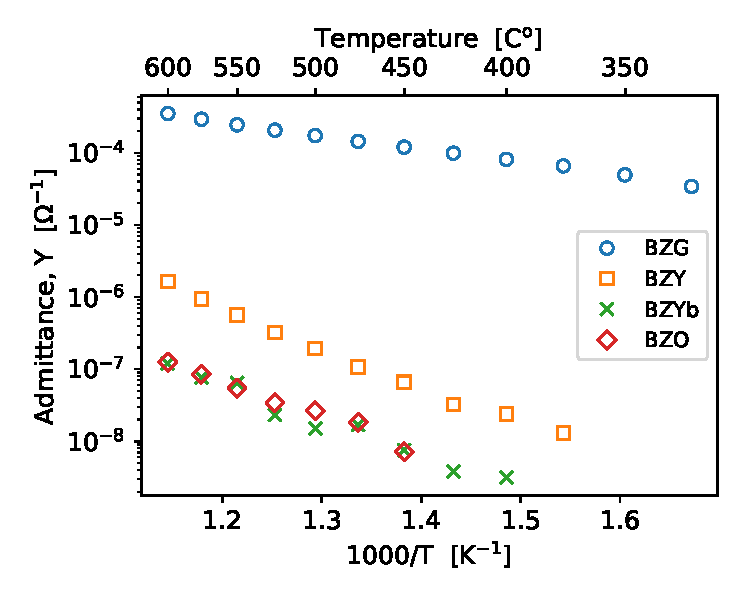
\includegraphics{Figures/190617-arr-admit-pellet-dopant-air.pdf}
\caption{Arrhenius-like plot of admittance over temperature comparing pellets made with different dopants. Pellets were made by solid state reaction. Impedance spectroscopy carried out under air atmosphere.}
\label{fig:bulk:arr:dopants}
\end{figure}

The bulk samples prepared with different dopants, that were analyzed by XRD, were then studied with impedance spectroscopy to evaluate the differences in conductivity as they pertained to dopant choice and by extension lattice constant. These pellets were all tested in air and had silver contacts applied in the ``in-plane'' geometry, shown in Figure \ref{fig:bulk:geometry}. Figure \ref{fig:bulk:arr:dopants} shows a strong effect that correlates with the results from lattice parameter shift in Figure \ref{fig:bulk:xrd:latticeParamDopantRadius}. The conductivity for undoped samples is very low, even at the low limit of the spectrometer's range to reliably measure impedance. Likewise, the ytterbium sample shows very poor conductivity, consistent with its potential levels of incorporation into the B site of the perovskite structure. Both yttrium and gadolinium show increased conductivity corresponding to their incorporation into the lattice and subsequent production of oxygen vacancies. 

In addition to this comparison of dopants using the ``in-plane'' geometry, measurements in the more typical ``through-plane'' geometry (see Figure \ref{fig:bulk:geometry}) were obtained in order to calculate conductivity itself over temperature and extract activation energies for these processes, as shown in Figure \ref{fig:bulk:arr:bzg_bzy}. These activation energies of gadolinium doped samples (0.65 eV) and yttrium doped samples (1.1 eV) are in the range consistent with the total conductivity (grain interior and grain boundary) of polycrystalline samples \cite{Gilardi2017}, although the conductivity is low particularly for the yttrium sample. In addition to the mechanism mentioned above of dopant incorporation, this sample is not fully dense and hardened as the gadolinium sample, with both suggesting more heat treatment is necessary in order to fully optimize conductivity for this bulk sample.
\begin{figure}
    \centering
    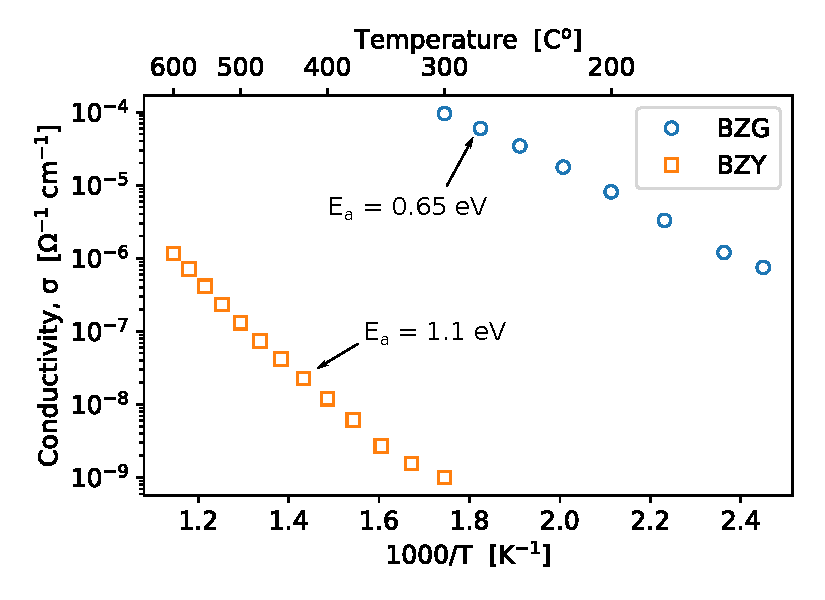
\includegraphics{Figures/190617-arr-bzg-bzy-thru-plane-air-edit.pdf}
    \caption{Arrhenius plots with BZG and BZY in the through plane geometry with conductivity calculated using the geometrical factor of each sample.}
    \label{fig:bulk:arr:bzg_bzy}
\end{figure}

\vspace{12pt}
\section{Conclusions}
Bulk samples of barium zirconate were synthesized by solid state reaction for the purpose of serving as ablation targets in the pulsed laser deposition system. These targets were produced according to established reactions and the process was monitored between steps by changes in X-ray diffraction patterns.

The pellets were made with a variety of dopants (Yb, Y, Gd), which, due to their difference in ionic radius, affect the lattice constant of the crystalline structure according to size. This change in lattice parameter was measured and while distortions were measured, this did not fall along a linear pattern as measured by others \cite{Gilardi2017}. This deviation was explained in terms of secondary phases either absent after the initial 1300\textdegree C reaction (in the case of Yb), or from the secondary phase still being present after the final 1600\textdegree C heat treatment. Both of these cases point to problems of dopant incorporation that manifest in changes in lattice parameter. 

Since these pellets were doped, conductivity measurements were recorded to serve as a point of comparison to the films which would be made from them. These conductivity measurements show gadolinium to be a promising material that may both incorporate better into the crystalline structure as well as promoted better conduction in its own right as suggested by Stokes \cite{Stokes2010} and Yamazaki \cite{Yamazaki2013}. 